\documentclass[tikz,border=8pt]{standalone}
\usepackage{tikz}
\usetikzlibrary{shapes,arrows,positioning}
\tikzstyle{proc}=[rectangle,draw,rounded corners,fill=blue!10,align=center,minimum width=3.4cm,minimum height=0.9cm,font=\small]
\tikzstyle{dec}=[diamond,draw,fill=green!10,align=center,aspect=2,font=\small]
\tikzstyle{term}=[rectangle,draw,rounded corners=8pt,fill=gray!15,align=center,minimum width=2.6cm,minimum height=0.9cm,font=\small\bfseries]
\tikzstyle{arr}=[->,thick]
\begin{document}
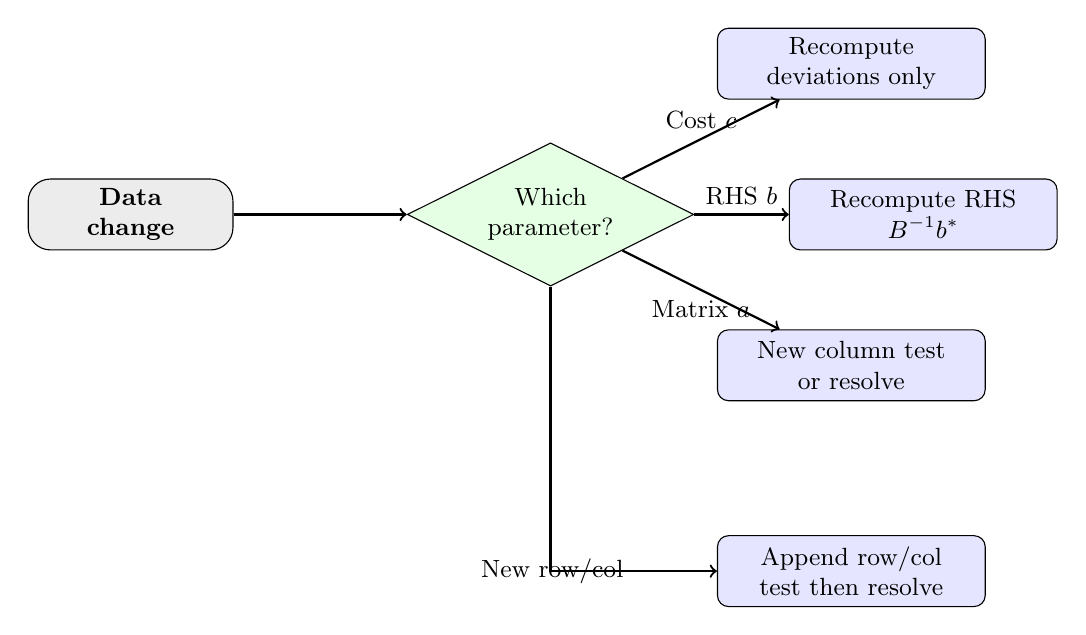
\begin{tikzpicture}[node distance=1.7cm]
\node (A) [term] {Data\\change};
\node (B) [dec, right=2.2cm of A] {Which\\parameter?};
\node (C) [proc, above right=1.0cm and 1.2cm of B] {Recompute\\deviations only};
\node (D) [proc, right=1.2cm of B] {Recompute RHS\\$B^{-1}b^*$};
\node (E) [proc, below right=1.0cm and 1.2cm of B] {New column test\\or resolve};
\node (F) [proc, below=of E] {Append row/col\\test then resolve};
\draw [arr] (A) -- (B);
\draw [arr] (B) -- node [above, font=\small] {Cost $c$} (C);
\draw [arr] (B) -- node [above, font=\small] {RHS $b$} (D);
\draw [arr] (B) -- node [below, font=\small] {Matrix $a$} (E);
\draw [arr] (B) |- node [left, font=\small, near end] {New row/col} (F);
\end{tikzpicture}
\end{document}
